\documentclass[aspectratio=169]{beamer}
\usepackage[utf8]{inputenc}

% design
\usetheme{CambridgeUS}
\usecolortheme{beaver}
\setbeamertemplate{itemize items}[square]
\usenavigationsymbolstemplate{\beamertemplatenavigationsymbolsempty}
\definecolor{darkred}{rgb}{0.8,0,0}
\setbeamertemplate{enumerate item}{\color{darkred}\insertenumlabel.}
\setbeamertemplate{itemize item}{\color{darkred}$\blacktriangleright$}
\setlength{\tabcolsep}{12pt}
\setbeamercolor{block title}{fg=darkred}

% bibliography
%\usepackage[backend=biber, style=authortitle]{biblatex}
\usepackage{natbib}
\usepackage{har2nat}
\bibliographystyle{unsrt}
%\addbibresource{../../smc.bib}
\usepackage{bibentry}
\nobibliography*

% tikz
\usepackage{tikz}
\usetikzlibrary{positioning}

% maths
\usepackage{amsmath}
\usepackage{amssymb}
\usepackage{amsfonts}
\usepackage{amsthm}
\theoremstyle{definition}
\newtheorem{defn}{Definition}

% useful math symbols
\newcommand{\PR}{\mathbb{P}}
\newcommand{\E}{\mathbb{E}}
\newcommand{\V}{\operatorname{Var}}
\newcommand{\eqdist}{\overset{d}{=}}
\newcommand{\I}[1]{\mathbb{I}\{#1\}}
\newcommand{\Ntoinfty}{\overset{N\to\infty}{\longrightarrow}}
\newcommand{\limNtoinfty}{\underset{N\to\infty}{\lim}}
\newcommand\indep{\protect\mathpalette{\protect\independenT}{\perp}}
\def\independenT#1#2{\mathrel{\rlap{$#1#2$}\mkern2mu{#1#2}}}

% distributions
\newcommand{\N}{\mathcal{N}}
\newcommand{\Cat}{\operatorname{Categorical}}
\newcommand{\Unif}{\operatorname{Uniform}}
\newcommand{\Mn}{\operatorname{Multinomial}}
\newcommand{\Bin}{\operatorname{Binomial}}

% project-specific commands
\newcommand{\F}{\mathcal{F}_{t-1}}
\newcommand{\vt}[2][t]{\nu_{#1}^{(#2)}}
%\newcommand{\vt}[1]{v_{#1}}
\newcommand{\wt}[2][t]{w_{#1}^{(#2)}}
%\newcommand{\wt}[1]{w_{#1}}
%\newcommand{\wbar}[2][t]{\bar{w}_{#1}^{(#2)}}
%\newcommand{\vttilde}[2][t]{\tilde{v}_{#1}^{(#2)}}
\newcommand{\Et}{\mathbb{E}_{t}}

\title[Genealogies of SMC Algorithms]{Asymptotic genealogies of sequential Monte Carlo algorithms}
\author[Suzie Brown]{\textbf{Suzie Brown} \\ with Paul Jenkins, Adam Johansen \& Jere Koskela}
\date{4 December 2020} 

\begin{document}
\begin{frame}
\maketitle
\end{frame}

\begin{frame}{Outline}
\begin{enumerate}
\item Sequential Monte Carlo
\item Resampling and degeneracy
\item SMC genealogies
\item Examples
\end{enumerate}
\end{frame}


\begin{frame}{Sequential Monte Carlo}
Approximate a sequence of distributions by simulating a population of particles evolving in time\\[10pt]
\pause
Iterate these steps:
\begin{enumerate}
\item \textbf{Mutate} particles via Markov transition density $q_t$
\item \textbf{Weight} particles by potential function $g_t$
\item \textbf{Resample} particles in proportion to their weights
\end{enumerate}
\end{frame}


\begin{frame}{Resampling}
\begin{columns}
\begin{column}{0.45\textwidth}
\onslide<1->
Stochastically map continuous weights $(\wt{1}, \dots, \wt{N})$ to discrete offspring counts $(\vt{1},\dots, \vt{N})$\\[10pt]
\onslide<2->
Properties:
\begin{itemize}
\item Number of particles constant $\sum_{i=1}^N \vt{i} =N$
\item Equal weights after resampling $w_{t+}^{(i)} = 1/N$
\item Unbiased\\ $\E[\vt{i} | \wt{1:N}] = N\wt{i}$
\end{itemize}

\end{column}
\begin{column}{0.45\textwidth}
\centering
\onslide<1->
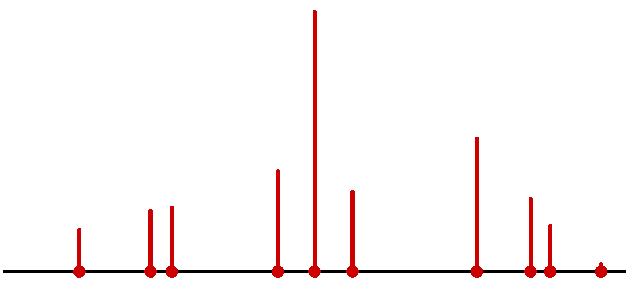
\includegraphics[width=\textwidth]{resample1.pdf} \\
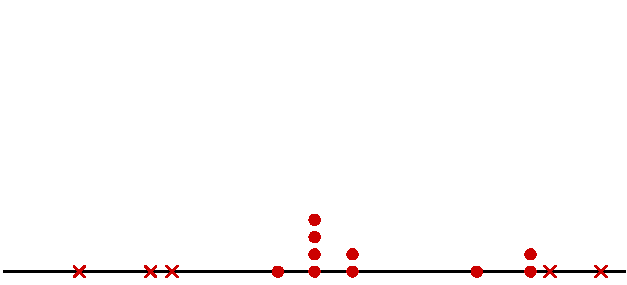
\includegraphics[width=\textwidth]{resample2.pdf}
\end{column}
\end{columns}
\end{frame}


\begin{frame}{Resampling induces a genealogy}
\centering
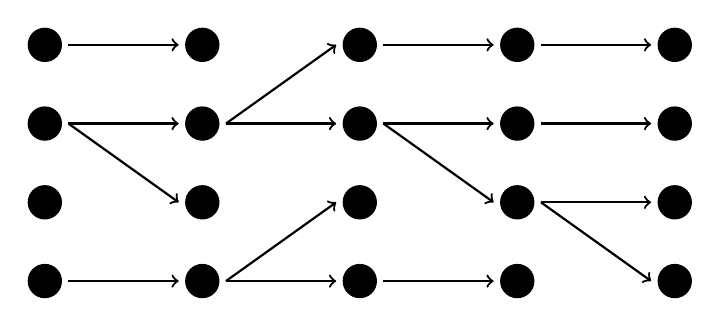
\begin{tikzpicture}
\filldraw (0,0) circle (6pt);
\filldraw (0,-1) circle (6pt);
\filldraw (0,-2) circle (6pt);
\filldraw (0,-3) circle (6pt);

\draw[->, thick] (0.3,0)--(1.7,0);
\draw[->, thick] (0.3,-1)--(1.7,-1);
\draw[->, thick] (0.3,-3)--(1.7,-3);
\draw[->, thick] (0.3,-1)--(1.7,-2);

\filldraw (2,0) circle (6pt);
\filldraw (2,-1) circle (6pt);
\filldraw (2,-2) circle (6pt);
\filldraw (2,-3) circle (6pt);

\pause

\filldraw (4,0) circle (6pt);
\filldraw (4,-1) circle (6pt);
\filldraw (4,-2) circle (6pt);
\filldraw (4,-3) circle (6pt);

\filldraw (6,0) circle (6pt);
\filldraw (6,-1) circle (6pt);
\filldraw (6,-2) circle (6pt);
\filldraw (6,-3) circle (6pt);

\filldraw (8,0) circle (6pt);
\filldraw (8,-1) circle (6pt);
\filldraw (8,-2) circle (6pt);
\filldraw (8,-3) circle (6pt);

\draw[->, thick] (2.3,-1)--(3.7,0);
\draw[->, thick] (2.3,-1)--(3.7,-1);
\draw[->, thick] (2.3,-3)--(3.7,-2);
\draw[->, thick] (2.3,-3)--(3.7,-3);

\draw[->, thick] (4.3,0)--(5.7,0);
\draw[->, thick] (4.3,-1)--(5.7,-1);
\draw[->, thick] (4.3,-1)--(5.7,-2);
\draw[->, thick] (4.3,-3)--(5.7,-3);

\draw[->, thick] (6.3,0)--(7.7,0);
\draw[->, thick] (6.3,-1)--(7.7,-1);
\draw[->, thick] (6.3,-2)--(7.7,-2);
\draw[->, thick] (6.3,-2)--(7.7,-3);
\end{tikzpicture}
\end{frame}


\begin{frame}{Resampling induces a genealogy}
\centering
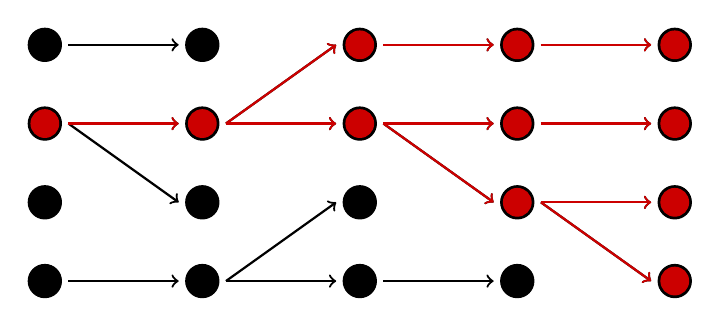
\begin{tikzpicture}
\filldraw (0,0) circle (6pt);
\filldraw (0,-1) circle (6pt);
\filldraw (0,-2) circle (6pt);
\filldraw (0,-3) circle (6pt);

\draw[->, thick] (0.3,0)--(1.7,0);
\draw[->, thick] (0.3,-1)--(1.7,-1);
\draw[->, thick] (0.3,-3)--(1.7,-3);
\draw[->, thick] (0.3,-1)--(1.7,-2);

\filldraw (2,0) circle (6pt);
\filldraw (2,-1) circle (6pt);
\filldraw (2,-2) circle (6pt);
\filldraw (2,-3) circle (6pt);

\filldraw (4,0) circle (6pt);
\filldraw (4,-1) circle (6pt);
\filldraw (4,-2) circle (6pt);
\filldraw (4,-3) circle (6pt);

\filldraw (6,0) circle (6pt);
\filldraw (6,-1) circle (6pt);
\filldraw (6,-2) circle (6pt);
\filldraw (6,-3) circle (6pt);

\filldraw (8,0) circle (6pt);
\filldraw (8,-1) circle (6pt);
\filldraw (8,-2) circle (6pt);
\filldraw (8,-3) circle (6pt);

\draw[->, thick] (2.3,-1)--(3.7,0);
\draw[->, thick] (2.3,-1)--(3.7,-1);
\draw[->, thick] (2.3,-3)--(3.7,-2);
\draw[->, thick] (2.3,-3)--(3.7,-3);

\draw[->, thick] (4.3,0)--(5.7,0);
\draw[->, thick] (4.3,-1)--(5.7,-1);
\draw[->, thick] (4.3,-1)--(5.7,-2);
\draw[->, thick] (4.3,-3)--(5.7,-3);

\draw[->, thick] (6.3,0)--(7.7,0);
\draw[->, thick] (6.3,-1)--(7.7,-1);
\draw[->, thick] (6.3,-2)--(7.7,-2);
\draw[->, thick] (6.3,-2)--(7.7,-3);

% highlight first lineage
\filldraw[darkred] (8,0) circle (5pt);
\pause
\filldraw[darkred] (6,0) circle (5pt);
\filldraw[darkred] (4,0) circle (5pt);
\filldraw[darkred] (2,-1) circle (5pt);
\filldraw[darkred] (0,-1) circle (5pt);

\draw[->, thick, darkred] (0.3,-1)--(1.7,-1);
\draw[->, thick, darkred] (2.3,-1)--(3.7,0);
\draw[->, thick, darkred] (4.3,0)--(5.7,0);
\draw[->, thick, darkred] (6.3,0)--(7.7,0);

\pause
% highlight other lineages
\filldraw[darkred] (4,-1) circle (5pt);
\filldraw[darkred] (6,-1) circle (5pt);
\filldraw[darkred] (8,-1) circle (5pt);
\filldraw[darkred] (6,-2) circle (5pt);
\filldraw[darkred] (8,-2) circle (5pt);
\filldraw[darkred] (8,-3) circle (5pt);

\draw[->, thick, darkred] (2.3,-1)--(3.7,-1);
\draw[->, thick, darkred] (4.3,-1)--(5.7,-1);
\draw[->, thick, darkred] (4.3,-1)--(5.7,-2);
\draw[->, thick, darkred] (6.3,-1)--(7.7,-1);
\draw[->, thick, darkred] (6.3,-2)--(7.7,-2);
\draw[->, thick, darkred] (6.3,-2)--(7.7,-3);
\end{tikzpicture}
\end{frame}


\begin{frame}{Resampling induces a genealogy}
\vspace{1cm}

\centering
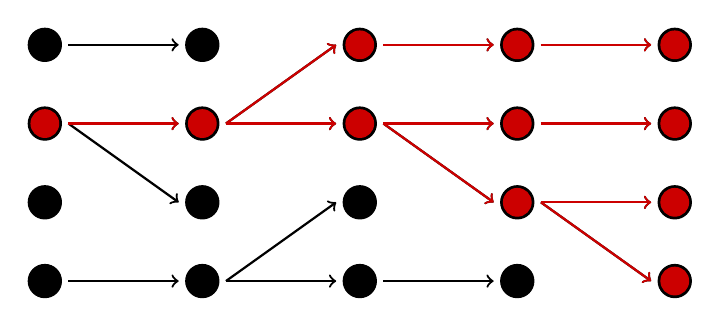
\begin{tikzpicture}
\filldraw (0,0) circle (6pt);
\filldraw (0,-1) circle (6pt);
\filldraw (0,-2) circle (6pt);
\filldraw (0,-3) circle (6pt);

\draw[->, thick] (0.3,0)--(1.7,0);
\draw[->, thick] (0.3,-1)--(1.7,-1);
\draw[->, thick] (0.3,-3)--(1.7,-3);
\draw[->, thick] (0.3,-1)--(1.7,-2);

\filldraw (2,0) circle (6pt);
\filldraw (2,-1) circle (6pt);
\filldraw (2,-2) circle (6pt);
\filldraw (2,-3) circle (6pt);

\filldraw (4,0) circle (6pt);
\filldraw (4,-1) circle (6pt);
\filldraw (4,-2) circle (6pt);
\filldraw (4,-3) circle (6pt);

\filldraw (6,0) circle (6pt);
\filldraw (6,-1) circle (6pt);
\filldraw (6,-2) circle (6pt);
\filldraw (6,-3) circle (6pt);

\filldraw (8,0) circle (6pt);
\filldraw (8,-1) circle (6pt);
\filldraw (8,-2) circle (6pt);
\filldraw (8,-3) circle (6pt);

\draw[->, thick] (2.3,-1)--(3.7,0);
\draw[->, thick] (2.3,-1)--(3.7,-1);
\draw[->, thick] (2.3,-3)--(3.7,-2);
\draw[->, thick] (2.3,-3)--(3.7,-3);

\draw[->, thick] (4.3,0)--(5.7,0);
\draw[->, thick] (4.3,-1)--(5.7,-1);
\draw[->, thick] (4.3,-1)--(5.7,-2);
\draw[->, thick] (4.3,-3)--(5.7,-3);

\draw[->, thick] (6.3,0)--(7.7,0);
\draw[->, thick] (6.3,-1)--(7.7,-1);
\draw[->, thick] (6.3,-2)--(7.7,-2);
\draw[->, thick] (6.3,-2)--(7.7,-3);

% highlight first lineage
\filldraw[darkred] (8,0) circle (5pt);
\filldraw[darkred] (6,0) circle (5pt);
\filldraw[darkred] (4,0) circle (5pt);
\filldraw[darkred] (2,-1) circle (5pt);
\filldraw[darkred] (0,-1) circle (5pt);

\draw[->, thick, darkred] (0.3,-1)--(1.7,-1);
\draw[->, thick, darkred] (2.3,-1)--(3.7,0);
\draw[->, thick, darkred] (4.3,0)--(5.7,0);
\draw[->, thick, darkred] (6.3,0)--(7.7,0);

% highlight other lineages
\filldraw[darkred] (4,-1) circle (5pt);
\filldraw[darkred] (6,-1) circle (5pt);
\filldraw[darkred] (8,-1) circle (5pt);
\filldraw[darkred] (6,-2) circle (5pt);
\filldraw[darkred] (8,-2) circle (5pt);
\filldraw[darkred] (8,-3) circle (5pt);

\draw[->, thick, darkred] (2.3,-1)--(3.7,-1);
\draw[->, thick, darkred] (4.3,-1)--(5.7,-1);
\draw[->, thick, darkred] (4.3,-1)--(5.7,-2);
\draw[->, thick, darkred] (6.3,-1)--(7.7,-1);
\draw[->, thick, darkred] (6.3,-2)--(7.7,-2);
\draw[->, thick, darkred] (6.3,-2)--(7.7,-3);
\end{tikzpicture}

\vspace{1cm}
\textbf{Ancestral degeneracy:} for $t<<T$, few distinct samples are available
\end{frame}


\begin{frame}{Mitigating ancestral degeneracy}
\vspace{-1cm}
Resample less often? \\
\pause
\textbf{Adaptive resampling}: only resample when effective sample size falls below some threshold.
\vspace{1cm}

\centering
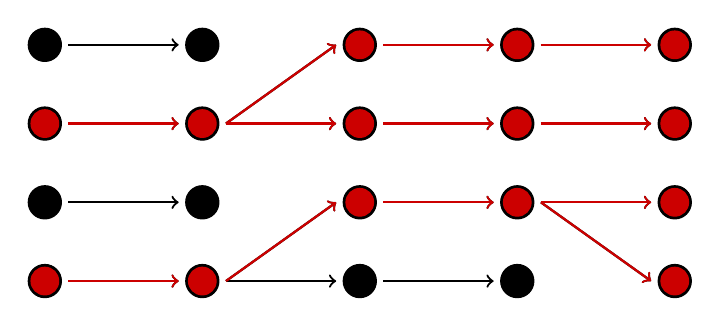
\begin{tikzpicture}
\filldraw (0,0) circle (6pt);
\filldraw (0,-1) circle (6pt);
\filldraw (0,-2) circle (6pt);
\filldraw (0,-3) circle (6pt);

\filldraw (2,0) circle (6pt);
\filldraw (2,-1) circle (6pt);
\filldraw (2,-2) circle (6pt);
\filldraw (2,-3) circle (6pt);

\filldraw (4,0) circle (6pt);
\filldraw (4,-1) circle (6pt);
\filldraw (4,-2) circle (6pt);
\filldraw (4,-3) circle (6pt);

\filldraw (6,0) circle (6pt);
\filldraw (6,-1) circle (6pt);
\filldraw (6,-2) circle (6pt);
\filldraw (6,-3) circle (6pt);

\filldraw (8,0) circle (6pt);
\filldraw (8,-1) circle (6pt);
\filldraw (8,-2) circle (6pt);
\filldraw (8,-3) circle (6pt);

\draw[->, thick] (0.3,0)--(1.7,0);
\draw[->, thick] (0.3,-1)--(1.7,-1);
\draw[->, thick] (0.3,-2)--(1.7,-2);
\draw[->, thick] (0.3,-3)--(1.7,-3);

\draw[->, thick] (2.3,-1)--(3.7,0);
\draw[->, thick] (2.3,-1)--(3.7,-1);
\draw[->, thick] (2.3,-3)--(3.7,-2);
\draw[->, thick] (2.3,-3)--(3.7,-3);

\draw[->, thick] (4.3,0)--(5.7,0);
\draw[->, thick] (4.3,-1)--(5.7,-1);
\draw[->, thick] (4.3,-2)--(5.7,-2);
\draw[->, thick] (4.3,-3)--(5.7,-3);

\draw[->, thick] (6.3,0)--(7.7,0);
\draw[->, thick] (6.3,-1)--(7.7,-1);
\draw[->, thick] (6.3,-2)--(7.7,-2);
\draw[->, thick] (6.3,-2)--(7.7,-3);

% highlight terminal particles, then each generation back in a block:
\filldraw[darkred] (8,0) circle (5pt);
\filldraw[darkred] (8,-1) circle (5pt);
\filldraw[darkred] (8,-2) circle (5pt);
\filldraw[darkred] (8,-3) circle (5pt);

\filldraw[darkred] (6,0) circle (5pt);
\filldraw[darkred] (6,-1) circle (5pt);
\filldraw[darkred] (6,-2) circle (5pt);

\filldraw[darkred] (4,0) circle (5pt);
\filldraw[darkred] (4,-1) circle (5pt);
\filldraw[darkred] (4,-2) circle (5pt);

\filldraw[darkred] (2,-1) circle (5pt);
\filldraw[darkred] (2,-3) circle (5pt);

\filldraw[darkred] (0,-1) circle (5pt);
\filldraw[darkred] (0,-3) circle (5pt);

% highlight arrows, starting at further right column:
\draw[->, thick, darkred] (6.3,0)--(7.7,0);
\draw[->, thick, darkred] (6.3,-1)--(7.7,-1);
\draw[->, thick, darkred] (6.3,-2)--(7.7,-2);
\draw[->, thick, darkred] (6.3,-2)--(7.7,-3);

\draw[->, thick, darkred] (4.3,0)--(5.7,0);
\draw[->, thick, darkred] (4.3,-1)--(5.7,-1);
\draw[->, thick, darkred] (4.3,-2)--(5.7,-2);

\draw[->, thick, darkred] (2.3,-1)--(3.7,0);
\draw[->, thick, darkred] (2.3,-1)--(3.7,-1);
\draw[->, thick, darkred] (2.3,-3)--(3.7,-2);

\draw[->, thick, darkred] (0.3,-1)--(1.7,-1);
\draw[->, thick, darkred] (0.3,-3)--(1.7,-3);
\end{tikzpicture}
\end{frame}


\begin{frame}{Mitigating ancestral degeneracy}
\vspace{-1cm}
Resample more cleverly? \\
\pause
\textbf{Low-variance resampling}: resample in a way that reduces the extra randomness added by the resampling step.
\vspace{1cm}

\centering
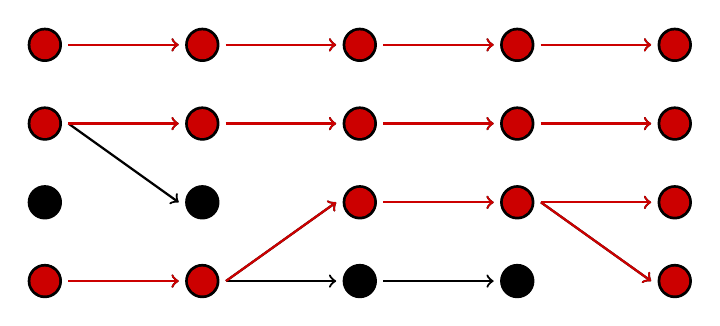
\begin{tikzpicture}
\filldraw (0,0) circle (6pt);
\filldraw (0,-1) circle (6pt);
\filldraw (0,-2) circle (6pt);
\filldraw (0,-3) circle (6pt);

\filldraw (2,0) circle (6pt);
\filldraw (2,-1) circle (6pt);
\filldraw (2,-2) circle (6pt);
\filldraw (2,-3) circle (6pt);

\filldraw (4,0) circle (6pt);
\filldraw (4,-1) circle (6pt);
\filldraw (4,-2) circle (6pt);
\filldraw (4,-3) circle (6pt);

\filldraw (6,0) circle (6pt);
\filldraw (6,-1) circle (6pt);
\filldraw (6,-2) circle (6pt);
\filldraw (6,-3) circle (6pt);

\filldraw (8,0) circle (6pt);
\filldraw (8,-1) circle (6pt);
\filldraw (8,-2) circle (6pt);
\filldraw (8,-3) circle (6pt);

\draw[->, thick] (0.3,0)--(1.7,0);
\draw[->, thick] (0.3,-1)--(1.7,-1);
\draw[->, thick] (0.3,-1)--(1.7,-2);
\draw[->, thick] (0.3,-3)--(1.7,-3);

\draw[->, thick] (2.3,0)--(3.7,0);
\draw[->, thick] (2.3,-1)--(3.7,-1);
\draw[->, thick] (2.3,-3)--(3.7,-2);
\draw[->, thick] (2.3,-3)--(3.7,-3);

\draw[->, thick] (4.3,0)--(5.7,0);
\draw[->, thick] (4.3,-1)--(5.7,-1);
\draw[->, thick] (4.3,-2)--(5.7,-2);
\draw[->, thick] (4.3,-3)--(5.7,-3);

\draw[->, thick] (6.3,0)--(7.7,0);
\draw[->, thick] (6.3,-1)--(7.7,-1);
\draw[->, thick] (6.3,-2)--(7.7,-2);
\draw[->, thick] (6.3,-2)--(7.7,-3);

% highlight terminal particles, then each generation back in a block:
\filldraw[darkred] (8,0) circle (5pt);
\filldraw[darkred] (8,-1) circle (5pt);
\filldraw[darkred] (8,-2) circle (5pt);
\filldraw[darkred] (8,-3) circle (5pt);

\filldraw[darkred] (6,0) circle (5pt);
\filldraw[darkred] (6,-1) circle (5pt);
\filldraw[darkred] (6,-2) circle (5pt);

\filldraw[darkred] (4,0) circle (5pt);
\filldraw[darkred] (4,-1) circle (5pt);
\filldraw[darkred] (4,-2) circle (5pt);

\filldraw[darkred] (2,0) circle (5pt);
\filldraw[darkred] (2,-1) circle (5pt);
\filldraw[darkred] (2,-3) circle (5pt);

\filldraw[darkred] (0,0) circle (5pt);
\filldraw[darkred] (0,-1) circle (5pt);
\filldraw[darkred] (0,-3) circle (5pt);

% highlight arrows, starting at further right column:
\draw[->, thick, darkred] (6.3,0)--(7.7,0);
\draw[->, thick, darkred] (6.3,-1)--(7.7,-1);
\draw[->, thick, darkred] (6.3,-2)--(7.7,-2);
\draw[->, thick, darkred] (6.3,-2)--(7.7,-3);

\draw[->, thick, darkred] (4.3,0)--(5.7,0);
\draw[->, thick, darkred] (4.3,-1)--(5.7,-1);
\draw[->, thick, darkred] (4.3,-2)--(5.7,-2);

\draw[->, thick, darkred] (2.3,0)--(3.7,0);
\draw[->, thick, darkred] (2.3,-1)--(3.7,-1);
\draw[->, thick, darkred] (2.3,-3)--(3.7,-2);

\draw[->, thick, darkred] (0.3,0)--(1.7,0);
\draw[->, thick, darkred] (0.3,-1)--(1.7,-1);
\draw[->, thick, darkred] (0.3,-3)--(1.7,-3);
\end{tikzpicture}
\end{frame}


\begin{frame}{Mitigating ancestral degeneracy}
\vspace{-1cm}
Make use of killed samples? \\
\pause
\textbf{Backward simulation}: use a backward pass to sample new ancestors for the terminal particles.
\vspace{1cm}

\centering
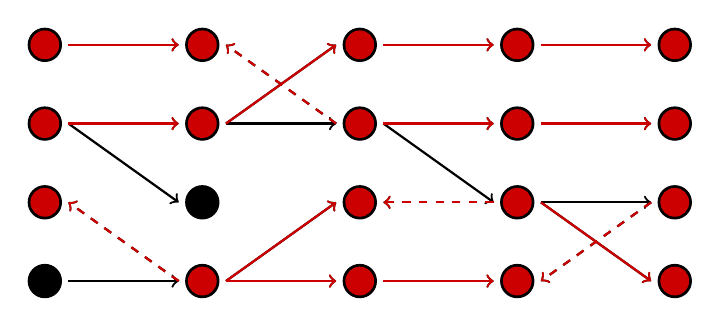
\begin{tikzpicture}
\filldraw (0,0) circle (6pt);
\filldraw (0,-1) circle (6pt);
\filldraw (0,-2) circle (6pt);
\filldraw (0,-3) circle (6pt);

\filldraw (2,0) circle (6pt);
\filldraw (2,-1) circle (6pt);
\filldraw (2,-2) circle (6pt);
\filldraw (2,-3) circle (6pt);

\filldraw (4,0) circle (6pt);
\filldraw (4,-1) circle (6pt);
\filldraw (4,-2) circle (6pt);
\filldraw (4,-3) circle (6pt);

\filldraw (6,0) circle (6pt);
\filldraw (6,-1) circle (6pt);
\filldraw (6,-2) circle (6pt);
\filldraw (6,-3) circle (6pt);

\filldraw (8,0) circle (6pt);
\filldraw (8,-1) circle (6pt);
\filldraw (8,-2) circle (6pt);
\filldraw (8,-3) circle (6pt);

\draw[->, thick] (0.3,0)--(1.7,0);
\draw[->, thick] (0.3,-1)--(1.7,-1);
\draw[->, thick] (0.3,-3)--(1.7,-3);
\draw[->, thick] (0.3,-1)--(1.7,-2);

\draw[->, thick] (2.3,-1)--(3.7,0);
\draw[->, thick] (2.3,-1)--(3.7,-1);
\draw[->, thick] (2.3,-3)--(3.7,-2);
\draw[->, thick] (2.3,-3)--(3.7,-3);

\draw[->, thick] (4.3,0)--(5.7,0);
\draw[->, thick] (4.3,-1)--(5.7,-1);
\draw[->, thick] (4.3,-1)--(5.7,-2);
\draw[->, thick] (4.3,-3)--(5.7,-3);

\draw[->, thick] (6.3,0)--(7.7,0);
\draw[->, thick] (6.3,-1)--(7.7,-1);
\draw[->, thick] (6.3,-2)--(7.7,-2);
\draw[->, thick] (6.3,-2)--(7.7,-3);

% backward simulation arrows
\draw[->, thick, dashed] (7.7,-2)--(6.3,-3);
\draw[->, thick, dashed] (5.7,-2)--(4.3,-2);
\draw[->, thick, dashed] (3.7,-1)--(2.3,0);
\draw[->, thick, dashed] (1.7,-3)--(0.3,-2);

% highlight terminal particles, then each generation back in a block:
\filldraw[darkred] (8,0) circle (5pt);
\filldraw[darkred] (8,-1) circle (5pt);
\filldraw[darkred] (8,-2) circle (5pt);
\filldraw[darkred] (8,-3) circle (5pt);

\filldraw[darkred] (6,0) circle (5pt);
\filldraw[darkred] (6,-1) circle (5pt);
\filldraw[darkred] (6,-2) circle (5pt);
\filldraw[darkred] (6,-3) circle (5pt);

\filldraw[darkred] (4,0) circle (5pt);
\filldraw[darkred] (4,-1) circle (5pt);
\filldraw[darkred] (4,-2) circle (5pt);
\filldraw[darkred] (4,-3) circle (5pt);

\filldraw[darkred] (2,0) circle (5pt);
\filldraw[darkred] (2,-1) circle (5pt);
\filldraw[darkred] (2,-3) circle (5pt);

\filldraw[darkred] (0,0) circle (5pt);
\filldraw[darkred] (0,-1) circle (5pt);
\filldraw[darkred] (0,-2) circle (5pt);

% highlight arrows, starting at further right column:
\draw[->, thick, darkred] (6.3,0)--(7.7,0);
\draw[->, thick, darkred] (6.3,-1)--(7.7,-1);
\draw[->, thick, darkred] (6.3,-2)--(7.7,-3);
\draw[->, thick, darkred, dashed] (7.7,-2)--(6.3,-3);

\draw[->, thick, darkred] (4.3,0)--(5.7,0);
\draw[->, thick, darkred] (4.3,-1)--(5.7,-1);
\draw[->, thick, darkred, dashed] (5.7,-2)--(4.3,-2);
\draw[->, thick, darkred] (4.3,-3)--(5.7,-3);

\draw[->, thick, darkred] (2.3,-1)--(3.7,0);
\draw[->, thick, darkred, dashed] (3.7,-1)--(2.3,0);
\draw[->, thick, darkred] (2.3,-3)--(3.7,-2);
\draw[->, thick, darkred] (2.3,-3)--(3.7,-3);

\draw[->, thick, darkred] (0.3,0)--(1.7,0);
\draw[->, thick, darkred] (0.3,-1)--(1.7,-1);
\draw[->, thick, darkred, dashed] (1.7,-3)--(0.3,-2);
\end{tikzpicture}
\end{frame}


\begin{frame}{Analysing genealogies}
\begin{itemize}
\item How many particles should I use to maintain $k$ distinct trajectories across time horizon $T$?
\item How big a lag can I use in fixed-lag smoothing?
\item How reliable is my smoothing estimator?
\item How do resampling schemes compare?
\end{itemize}
\end{frame}


\begin{frame}{Encoding genealogies}
\centering
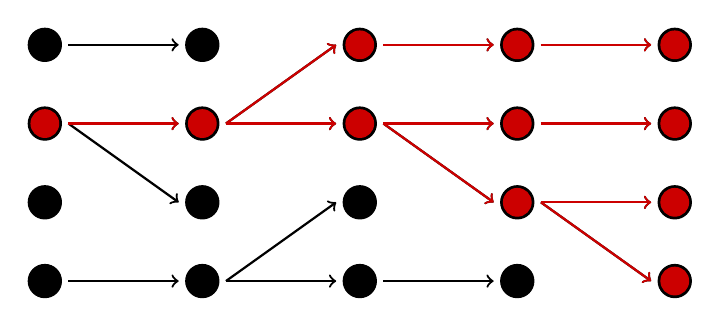
\begin{tikzpicture}
\filldraw (0,0) circle (6pt);
\filldraw (0,-1) circle (6pt);
\filldraw (0,-2) circle (6pt);
\filldraw (0,-3) circle (6pt);

\draw[->, thick] (0.3,0)--(1.7,0);
\draw[->, thick] (0.3,-1)--(1.7,-1);
\draw[->, thick] (0.3,-3)--(1.7,-3);
\draw[->, thick] (0.3,-1)--(1.7,-2);

\filldraw (2,0) circle (6pt);
\filldraw (2,-1) circle (6pt);
\filldraw (2,-2) circle (6pt);
\filldraw (2,-3) circle (6pt);

\filldraw (4,0) circle (6pt);
\filldraw (4,-1) circle (6pt);
\filldraw (4,-2) circle (6pt);
\filldraw (4,-3) circle (6pt);

\filldraw (6,0) circle (6pt);
\filldraw (6,-1) circle (6pt);
\filldraw (6,-2) circle (6pt);
\filldraw (6,-3) circle (6pt);

\filldraw (8,0) circle (6pt);
\filldraw (8,-1) circle (6pt);
\filldraw (8,-2) circle (6pt);
\filldraw (8,-3) circle (6pt);

\draw[->, thick] (2.3,-1)--(3.7,0);
\draw[->, thick] (2.3,-1)--(3.7,-1);
\draw[->, thick] (2.3,-3)--(3.7,-2);
\draw[->, thick] (2.3,-3)--(3.7,-3);

\draw[->, thick] (4.3,0)--(5.7,0);
\draw[->, thick] (4.3,-1)--(5.7,-1);
\draw[->, thick] (4.3,-1)--(5.7,-2);
\draw[->, thick] (4.3,-3)--(5.7,-3);

\draw[->, thick] (6.3,0)--(7.7,0);
\draw[->, thick] (6.3,-1)--(7.7,-1);
\draw[->, thick] (6.3,-2)--(7.7,-2);
\draw[->, thick] (6.3,-2)--(7.7,-3);

% highlight first lineage
\filldraw[darkred] (8,0) circle (5pt);
\filldraw[darkred] (6,0) circle (5pt);
\filldraw[darkred] (4,0) circle (5pt);
\filldraw[darkred] (2,-1) circle (5pt);
\filldraw[darkred] (0,-1) circle (5pt);

\draw[->, thick, darkred] (0.3,-1)--(1.7,-1);
\draw[->, thick, darkred] (2.3,-1)--(3.7,0);
\draw[->, thick, darkred] (4.3,0)--(5.7,0);
\draw[->, thick, darkred] (6.3,0)--(7.7,0);

% highlight other lineages
\filldraw[darkred] (4,-1) circle (5pt);
\filldraw[darkred] (6,-1) circle (5pt);
\filldraw[darkred] (8,-1) circle (5pt);
\filldraw[darkred] (6,-2) circle (5pt);
\filldraw[darkred] (8,-2) circle (5pt);
\filldraw[darkred] (8,-3) circle (5pt);

\draw[->, thick, darkred] (2.3,-1)--(3.7,-1);
\draw[->, thick, darkred] (4.3,-1)--(5.7,-1);
\draw[->, thick, darkred] (4.3,-1)--(5.7,-2);
\draw[->, thick, darkred] (6.3,-1)--(7.7,-1);
\draw[->, thick, darkred] (6.3,-2)--(7.7,-2);
\draw[->, thick, darkred] (6.3,-2)--(7.7,-3);
\end{tikzpicture}
\end{frame}


\begin{frame}{Encoding genealogies}
\centering
\begin{tikzpicture}
\draw[dotted] (0,-4.5)--(0,0.5);
\draw[dotted] (2,-4.5)--(2,0.5);
\draw[dotted] (4,-4.5)--(4,0.5);
\draw[dotted] (6,-4.5)--(6,0.5);
\draw[dotted] (8,-4.5)--(8,0.5);

\draw[thick, darkred] (0,-1)--(2,-1);
\draw[thick, darkred] (2,0)--(2,-2);
\draw[thick, darkred] (2,0)--(8,0);
\draw[thick, darkred] (2,-2)--(4,-2);
\draw[thick, darkred] (4,-3)--(4,-1);
\draw[thick, darkred] (4,-1)--(8,-1);
\draw[thick, darkred] (4,-3)--(6,-3);
\draw[thick, darkred] (6,-2)--(6,-4);
\draw[thick, darkred] (6,-2)--(8,-2);
\draw[thick, darkred] (6,-4)--(8,-4);
%
%\node at (8.3,0) {1};
%\node at (8.3,-1) {2};
%\node at (8.3,-2) {3};
%\node at (8.3,-4) {4};
\end{tikzpicture}
\end{frame}


\begin{frame}{Encoding genealogies}
\begin{itemize}
\item Label time in reverse
\pause
\item Population of $N$ particles
\item Sample $n\leq N$ terminal particles at random
\pause
\item Describe genealogy by stochastic process $(G_t^{(n,N)})_{t\in\mathbb{N}_0}$ on space of partitions of $\{1,\dots,n\}$
\item Elements $i, j$ are in the same block of the partition $G_t^{(n,N)}$ iff particles $i$ and $j$ share a common ancestor at time $t$
\pause
\item Initially $G_0^{(n,N)} = \{ \{1\}, \dots, \{n\} \}$
\item The only possible non-identity transitions are those that merge blocks
\item The trivial partition $\{ \{ 1,\dots, n \} \}$ is an absorbing state
\end{itemize}
\end{frame}


\begin{frame}{Encoding genealogies}
\centering
\begin{tikzpicture}
\draw[dotted] (0,-4.5)--(0,0.5);
\draw[dotted] (2,-4.5)--(2,0.5);
\draw[dotted] (4,-4.5)--(4,0.5);
\draw[dotted] (6,-4.5)--(6,0.5);
\draw[dotted] (8,-4.5)--(8,0.5);

\draw[thick, darkred] (0,-1)--(2,-1);
\draw[thick, darkred] (2,0)--(2,-2);
\draw[thick, darkred] (2,0)--(8,0);
\draw[thick, darkred] (2,-2)--(4,-2);
\draw[thick, darkred] (4,-3)--(4,-1);
\draw[thick, darkred] (4,-1)--(8,-1);
\draw[thick, darkred] (4,-3)--(6,-3);
\draw[thick, darkred] (6,-2)--(6,-4);
\draw[thick, darkred] (6,-2)--(8,-2);
\draw[thick, darkred] (6,-4)--(8,-4);

\node at (8.3,0) {1};
\node at (8.3,-1) {2};
\node at (8.3,-2) {3};
\node at (8.3,-4) {4};

\pause

\node at (8,-4.8) {$t=0$};
\node at (8,-5.5) {$\{1\}, \{2\},\{3\}, \{4\}$};
\end{tikzpicture}
\end{frame}

\begin{frame}{Encoding genealogies}
\centering
\begin{tikzpicture}
\draw[dotted] (0,-4.5)--(0,0.5);
\draw[dotted] (2,-4.5)--(2,0.5);
\draw[dotted] (4,-4.5)--(4,0.5);
\draw[dotted] (6,-4.5)--(6,0.5);
\draw[dotted] (8,-4.5)--(8,0.5);

\draw[thick, darkred] (0,-1)--(2,-1);
\draw[thick, darkred] (2,0)--(2,-2);
\draw[thick, darkred] (2,0)--(8,0);
\draw[thick, darkred] (2,-2)--(4,-2);
\draw[thick, darkred] (4,-3)--(4,-1);
\draw[thick, darkred] (4,-1)--(8,-1);
\draw[thick, darkred] (4,-3)--(6,-3);
\draw[thick, darkred] (6,-2)--(6,-4);
\draw[thick, darkred] (6,-2)--(8,-2);
\draw[thick, darkred] (6,-4)--(8,-4);

\node at (8.3,0) {1};
\node at (8.3,-1) {2};
\node at (8.3,-2) {3};
\node at (8.3,-4) {4};

\node at (6,-4.8) {$t=1$};
\node at (6,-5.5) {$\{1\}, \{2\},\{3,4\}$};
\end{tikzpicture}
\end{frame}

\begin{frame}{Encoding genealogies}
\centering
\begin{tikzpicture}
\draw[dotted] (0,-4.5)--(0,0.5);
\draw[dotted] (2,-4.5)--(2,0.5);
\draw[dotted] (4,-4.5)--(4,0.5);
\draw[dotted] (6,-4.5)--(6,0.5);
\draw[dotted] (8,-4.5)--(8,0.5);

\draw[thick, darkred] (0,-1)--(2,-1);
\draw[thick, darkred] (2,0)--(2,-2);
\draw[thick, darkred] (2,0)--(8,0);
\draw[thick, darkred] (2,-2)--(4,-2);
\draw[thick, darkred] (4,-3)--(4,-1);
\draw[thick, darkred] (4,-1)--(8,-1);
\draw[thick, darkred] (4,-3)--(6,-3);
\draw[thick, darkred] (6,-2)--(6,-4);
\draw[thick, darkred] (6,-2)--(8,-2);
\draw[thick, darkred] (6,-4)--(8,-4);

\node at (8.3,0) {1};
\node at (8.3,-1) {2};
\node at (8.3,-2) {3};
\node at (8.3,-4) {4};

\node at (4,-4.8) {$t=2$};
\node at (4,-5.5) {$\{1\}, \{2,3,4\}$};
\end{tikzpicture}
\end{frame}

\begin{frame}{Encoding genealogies}
\centering
\begin{tikzpicture}
\draw[dotted] (0,-4.5)--(0,0.5);
\draw[dotted] (2,-4.5)--(2,0.5);
\draw[dotted] (4,-4.5)--(4,0.5);
\draw[dotted] (6,-4.5)--(6,0.5);
\draw[dotted] (8,-4.5)--(8,0.5);

\draw[thick, darkred] (0,-1)--(2,-1);
\draw[thick, darkred] (2,0)--(2,-2);
\draw[thick, darkred] (2,0)--(8,0);
\draw[thick, darkred] (2,-2)--(4,-2);
\draw[thick, darkred] (4,-3)--(4,-1);
\draw[thick, darkred] (4,-1)--(8,-1);
\draw[thick, darkred] (4,-3)--(6,-3);
\draw[thick, darkred] (6,-2)--(6,-4);
\draw[thick, darkred] (6,-2)--(8,-2);
\draw[thick, darkred] (6,-4)--(8,-4);

\node at (8.3,0) {1};
\node at (8.3,-1) {2};
\node at (8.3,-2) {3};
\node at (8.3,-4) {4};

\node at (2,-4.8) {$t=3$};
\node at (2,-5.5) {$\{1,2,3,4\}$};
\end{tikzpicture}
\end{frame}


\begin{frame}{Kingman's $n$-coalescent\footnote[frame]{J F C Kingman, \textit{Stochastic Processes \& their Applications}, 1982.}}
\begin{columns}
\begin{column}{0.45\textwidth}
\begin{itemize}
\item Continuous-time Markov chain on the space of partitions of $\{1,\dots,n\}$
\item Single pair mergers only
\item Each pair merges independently at rate 1 (total merge rate $\binom{k}{2}$ while there are $k$ distinct lineages)
\end{itemize}
\end{column}
\begin{column}{0.45\textwidth}
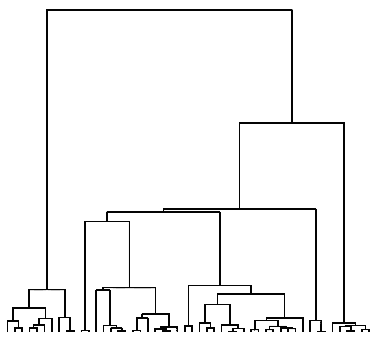
\includegraphics[width=\textwidth]{kingman.png}
\hspace*{\fill} \tiny{image: Wikimedia Commons}
\end{column}
\end{columns}
\end{frame}


\begin{frame}{Time scale}
Pair merger probability conditional on $( \vt{1},\dots, \vt{N} )$:
\begin{equation*}
c_N(t) = \frac{1}{(N)_2} \sum_{i=1}^N (\vt{i})_2
\end{equation*}
\pause
Rescale time by inverse:
\begin{equation*}
\tau_N(t) := \inf\left\{ s\geq 1 : \sum_{r=1}^s c_N(r) \geq t \right\}
\end{equation*}
\end{frame}


\begin{frame}{Main theorem}
Conditions:
\begin{itemize}
\item Parent-offspring assignments are uniform given offspring counts
\pause
\item Time scale does not explode (i.e.\ $\PR[\tau_N(t)=\infty]=0$ for all finite $t$)
\pause
\item There exists a sequence $(b_N)$ such that $\lim_{N\to\infty} b_N = 0$ and
\begin{equation*}
\frac{1}{(N)_3} \sum_{i=1}^N \E_t [ (\vt{i})_3 ]
\leq b_N \frac{1}{(N)_2} \sum_{i=1}^N \E_t [ (\vt{i})_2 ]
\end{equation*}
\end{itemize}
\pause
Then the finite-dimensional distributions of the time-rescaled genealogies $\left( G_{\tau_N(t)}^{(n,N)} \right)_{t\geq0}$ converge to Kingman's $n$-coalescent as $N\to\infty$.
\end{frame}


\begin{frame}{Examples}
\begin{itemize}
\item Multinomial resampling
\item Stochastic rounding 
\item Conditional SMC with multinomial resampling
\end{itemize}
\end{frame}


\begin{frame}{Multinomial resampling}
Resample from a Categorical distribution, so offspring counts are Multinomial:
\begin{equation*}
(\vt{1} , \dots, \vt{N}) \sim \Mn \left( N, (\wt{1},\dots,\wt{N}) \right)
\end{equation*}
\pause
Suppose the potentials $g_t$ and transition densities $q_t$ satisfy
\begin{equation*}
\frac{1}{a} \leq g_t(x, x^\prime) \leq a \qquad
\varepsilon h(x^\prime) \leq q_t(x, x^\prime) \leq \frac{1}{\varepsilon} h(x^\prime) 
\end{equation*}
for constants $0<\varepsilon\leq 1\leq a<\infty$, and probability distribution $h(\cdot)$.\\[10pt]
\pause
Then the rescaled genealogies converge to the $n$-coalescent.\footnote{J Koskela, PA Jenkins, AM Johansen, D Span\`o. \textit{Annals of Statistics}, 2020.}
\end{frame}


\begin{frame}{Stochastic rounding}
$\mathbf{Y}: \mathbb{R}_+^N \to \mathbb{N}^N$ is a \emph{stochastic rounding} of $\mathbf{X}$ if for $i=1,\dots,N$
\begin{equation*}
Y_i \mid X_i =
\begin{cases}
 \lfloor X_i \rfloor & \text{with probability } 1- X_i + \lfloor X_i \rfloor \\
  \lfloor X_i \rfloor +1 & \text{with probability } X_i - \lfloor X_i \rfloor 
\end{cases}
\end{equation*}
\pause
\begin{itemize}
\item Take $X_i = N\wt{i}$ and $Y_i = \vt{i}$
\item By construction $\E[Y_i \mid \mathbf{X}] = X_i$
\item Require further constraint $Y_1 + \cdots + Y_N = N$
\pause
\item \textbf{Examples:} systematic, residual-stratified, branching system\footnote{D Crisan, T Lyons. \textit{Probability Theory \& Related Fields}, 1997.}, SSP\footnote{M Gerber, N Whiteley, N Chopin. \textit{Annals of Statistics}, 2019.} resampling
\end{itemize}
\end{frame}


\begin{frame}{Stochastic rounding}
Resample using any stochastic rounding procedure.\\[10pt]
\pause
Suppose the potentials $g_t$ and transition densities $q_t$ satisfy
\begin{equation*}
\frac{1}{a} \leq g_t(x, x^\prime) \leq a \qquad
\varepsilon \leq q_t(x, x^\prime) \leq \frac{1}{\varepsilon} 
\end{equation*}
for constants $0<\varepsilon\leq 1\leq a<\infty$.\\[10pt]
\pause
Then the rescaled genealogies converge to the $n$-coalescent.
\end{frame}


\begin{frame}{Conditional SMC}
A particle Gibbs\footnote{C Andrieu, A Doucet, R Holenstein. \textit{Journal of the Royal Statistical Society B}, 2010.} scenario...
\begin{itemize}[<+->]
\item Want to target $p(\theta, x_{0:T} \mid y_{0:T})$
\item Gibbs sampler: alternate samples from \\
\hspace{1cm} $p(\theta \mid x_{0:T}, y_{0:T})$ (easy) and \\
\hspace{1cm} $p(x_{0:T} \mid \theta, y_{0:T})$ (using SMC)
\item Standard SMC updates don't target the correct distribution
\item Use SMC updates that are \emph{conditioned} on the previous $X_{0:T}$ trajectory (states and ancestors)
\item Resampling must deterministically propagate this ``immortal lineage''
%\item Ancestral degeneracy prevents the chain mixing on $x_{0:t}$
\end{itemize}
\end{frame}


\begin{frame}{Conditional SMC}
\begin{columns}
\begin{column}{0.45\textwidth}
\centering
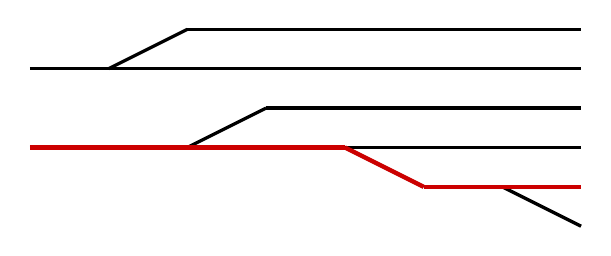
\begin{tikzpicture}
% horizontals
\draw[very thick] (0,1)--(7,1);
\draw[very thick] (2,1.5)--(7,1.5);
\draw[very thick] (3,0.5)--(7,0.5);
\draw[very thick] (0,0)--(7,0);
\draw[very thick] (5,-0.5)--(7,-0.5);
% diagonals
\draw[very thick] (1,1)--(2,1.5);
\draw[very thick] (2,0)--(3,0.5);
\draw[very thick] (4,0)--(5,-0.5);
\draw[very thick] (6,-0.5)--(7,-1);
% red highlight:
\draw[darkred, ultra thick] (0,0)--(4,0);
\draw[darkred, ultra thick] (5,-0.5)--(7,-0.5);
\draw[darkred, ultra thick] (4,0)--(5,-0.5);
\end{tikzpicture}
\pause
okay
\end{column}
\begin{column}{0.45\textwidth}
\centering
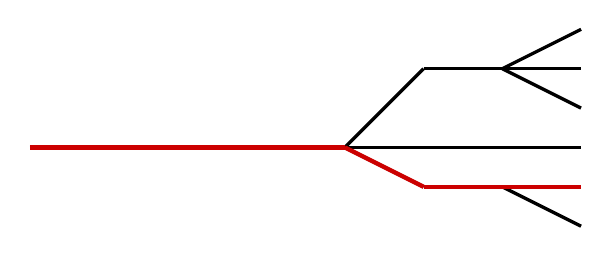
\begin{tikzpicture}
% horizontals
\draw[very thick] (5,1)--(7,1);
\draw[very thick] (0,0)--(7,0);
\draw[very thick] (5,-0.5)--(7,-0.5);
% diagonals
\draw[very thick] (6,1)--(7,1.5);
\draw[very thick] (6,1)--(7,0.5);
\draw[very thick] (4,0)--(5,1);
\draw[very thick] (4,0)--(5,-0.5);
\draw[very thick] (6,-0.5)--(7,-1);
% red highlight:
\draw[darkred, ultra thick] (0,0)--(4,0);
\draw[darkred, ultra thick] (5,-0.5)--(7,-0.5);
\draw[darkred, ultra thick] (4,0)--(5,-0.5);
\end{tikzpicture}

not okay
\end{column}
\end{columns}
\end{frame}


\begin{frame}{Conditional SMC}
Consider a conditional SMC algorithm with multinomial resampling.\\[10pt]
\pause
Assume
\begin{equation*}
\frac{1}{a} \leq g_t(x, x^\prime) \leq a \qquad
\varepsilon h(x^\prime) \leq q_t(x, x^\prime) \leq \frac{1}{\varepsilon} h(x^\prime) .
\end{equation*}

\pause
Then the rescaled genealogies converge to the $n$-coalescent.
\end{frame}


\begin{frame}{Quantities of interest}
\begin{columns}
\begin{column}{0.45\textwidth}
\begin{itemize}[<+->]
\item Time to MRCA: first time when there is only one distinct lineage
\item $T_k$: time interval where there are exactly $k$ distinct lineages
\item Total branch length: storage cost
\end{itemize}
\end{column}
\begin{column}{0.45\textwidth}
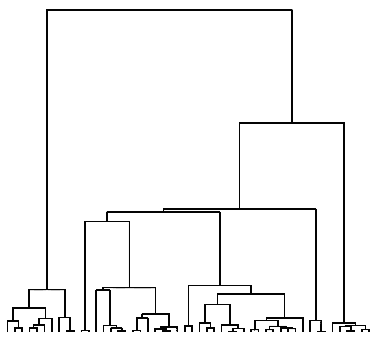
\includegraphics[width=\textwidth]{kingman.png}
\hspace*{\fill} \tiny{image: Wikimedia Commons}
\end{column}
\end{columns}
\end{frame}


\begin{frame}{Mitigating ancestral degeneracy, revisited}
\pause
\begin{itemize}[<+->]
\item \textbf{Adaptive resampling}: should slow down the time-scale on which the coalescent is recovered (it may have some other effect)
\item \textbf{Low-variance resampling}: stochastic rounding schemes have minimal variance
\item \textbf{Backward simulation}: the backward-in-time process is not a pure coalescent, and is not induced by resampling
\end{itemize}
\end{frame}


\begin{frame}{In conclusion...}
\begin{itemize}
\item Genealogies can help us to analyse performance of SMC algorithms which suffer ancestral degeneracy
\item We have simple conditions under which these genealogies converge to Kingman's $n$-coalescent
\item These conditions are verified for some important classes of SMC algorithms
\end{itemize}
\end{frame}


\begin{frame}{Open questions}
\begin{itemize}
\item Weak convergence
\item Other resampling schemes (stratified, residual-multinomial, ...)
\item Effect of adaptive resampling
\item Estimating the time scale $\tau_N$ a priori (since it depends on observed offspring counts)
\item Finite-$N$ behaviour
\end{itemize}
\end{frame}


\begin{frame}
\centering
\vspace{1cm}
{\Large Thank you!}\\
\vspace{1cm}
pre-print at arXiv:2007.00096
\end{frame}


\end{document}